\section{Introduction}

Evolutionary biology is driven by two mathematically distinct mechanisms: vertical descent, characterized by the gradual accumulation of point mutations over time (clonal expansion), and horizontal exchange, where distinct genetic lineages undergo rapid, macro-evolutionary mixing (reticulation). This horizontal exchange is not a statistical anomaly but rather the primary driver of rapid adaptation and immune evasion \citep{simon2015hiv}. In segmented RNA viruses such as Influenza A, genomic reassortment allows entirely novel strains to emerge through the exchange of entire genomic segments between co-infecting viruses---a mechanism responsible for nearly all major influenza pandemics, including the devastating triple-reassortant H7N9 avian influenza \citep{nelson2014emergence}. Similarly, retroviruses like HIV-1 frequently undergo homologous recombination during reverse transcription, generating circulating recombinant forms (CRFs) that rapidly acquire multi-drug resistance and evade host immunity \citep{simon2015hiv}. In bacterial populations, horizontal gene transfer (HGT) facilitates the immediate, non-lineal acquisition of virulence factors across entirely distinct species, effectively bypassing the slow clock of vertical evolution. Furthermore, in DNA viruses such as the Hepatitis B Virus (HBV), homologous recombination across overlapping open reading frames introduces profound structural dependencies that linear evolutionary models fundamentally misinterpret \citep{zhou2012recombination}.

Despite the absolute biological centrality of reticulation, the computational interpretation of evolutionary history has historically been tethered to the rigid conceptual framework of the strictly bifurcating tree. Originating as a heuristic representation of vertical descent, this directed acyclic graph (DAG) model forms the foundational axiom for modern phylogenetic algorithms, ranging from primitive Neighbor-Joining distance matrices to advanced Maximum Likelihood and Bayesian inference frameworks \citep{felsenstein1981evolutionary, nguyen2015iq, stamatakis2014raxml, suchard2018bayesian}. Within these established frameworks---including industry standards such as IQ-TREE \citep{nguyen2015iq}, RAxML \citep{stamatakis2014raxml}, and BEAST \citep{suchard2018bayesian}---speciation or viral divergence is mathematically constrained to a node splitting into exactly two distinct, divergent lineages. 

When reticulate evolution occurs, genomic lineages do not merely diverge; they converge, exchange material, and merge, forming physical and biological loops. Attempting to force a recombinant or reassortant genomic sequence into a strictly bifurcating phylogenetic algorithm results in severe biological and topological distortions. Because these algorithms are mathematically blind to convergent loops, they attempt to resolve the evolutionary contradictions by hallucinating false ancestral nodes, artificially inflating branch lengths, or placing the recombinant lineages at wildly inaccurate positions near the root of the tree \citep{huson2006application}. Consequently, the reliance on bifurcating models for highly reticulate viral populations fundamentally misrepresents the underlying biology. It compromises epidemiological tracking, obscures the true biological origins of vaccine-escape variants, and yields geometrically incorrect evolutionary trajectories. While phylogenetic network models, such as splits graphs \citep{huson2006application}, have been developed to address this glaring deficiency, they frequently rely on computationally expensive, ad-hoc combinatorial heuristics that lack a rigorous metric space definition, making them virtually impossible to scale and highly prone to overfitting noisy alignments generated by software like MAFFT \citep{katoh2013mafft}. Furthermore, metrics built on top of these trees, such as the standard dN/dS ratio for selective pressure, collapse mathematically when applied to overlapping ORFs (e.g., in HBV), where synonymous mutations in one frame are necessarily non-synonymous in another \citep{schlub2018estimating}.

To resolve the mathematical incompatibility between bifurcating trees and the biological reality of reticulation, mathematicians have turned to Topological Data Analysis (TDA) \citep{carlsson2009topology, lum2013extracting}. TDA abandons the assumption of a predefined graph structure entirely. Instead, it treats genomic sequences as a multidimensional point cloud embedded in a formal metric space. The pioneering application of TDA to viral evolution was established by Chan, Carlsson, and Rabadan in their seminal work \textit{Topology of Viral Evolution}, which introduced Persistent Homology as a rigorous geometric tool to explicitly detect reassortment \citep{chan2013topology}. Rather than forcing sequences into an arbitrary tree, persistent homology evaluates the topological features of the data across multiple distance scales, known as filtrations \citep{edelsbrunner2000topological, zomorodian2005computing}. In this framework, vertical, clonal evolution is geometrically classified as zero-dimensional homology ($H_0$), representing isolated data components merging into a single connected component (a tree-like structure). Conversely, reticulate evolutionary events---such as Influenza reassortment and HIV recombination---manifest mathematically as one-dimensional topological holes or loops ($H_1$). By tracking the birth and death of these $H_1$ features, Rabadan and colleagues proved that reticulate biology generates a distinct, non-trivial topological signature that is entirely invisible to standard phylogenetic trees \citep{chan2013topology}.

While the mathematical rigor of persistent homology provides an elegant, exact solution to the bifurcation problem, its empirical deployment in modern bioinformatics has been severely hindered by catastrophic computational bottlenecks. The standard construction of the Vietoris-Rips complex, absolutely necessary to compute $H_1$ persistence, scales exponentially ($O(2^N)$) with the number of sequences \citep{bauer2021ripser}. Previous TDA implementations, frequently authored as inefficient Python \citep{van1995python} or R \citep{r2024} wrappers around generic algebraic topology libraries, encounter devastating memory exhaustion when presented with even moderately sized viral datasets. As a direct result of these software engineering failures, TDA in phylogenetics has largely been restricted to theoretical proofs-of-concept or small, heavily down-sampled alignments \citep{bauer2021ripser}, leaving the broader bioinformatics industry inextricably bound to the computationally faster, yet biologically inaccurate, bifurcating tree algorithms.

In this manuscript, I present ATLAZ (Alignment, Topology, and Lineage Analysis in Zig), a production-grade, memory-deterministic geometric engine written entirely in the systems-level Zig programming language \citep{zig2024}, acting as a topological subcomponent of the broader BioZig ecosystem. ATLAZ completely resolves the bifurcation axiom by deploying a zero-copy C-ABI boundary and native Galois Field (GF(2)) matrix reductions. I rigorously validate the engine against empirical viral datasets, demonstrating its capacity to rapidly confirm clonal, tree-like vertical descent in outbreaks like Ebola \citep{kuiken2012lanl}, while simultaneously exposing the dense, reticulate $H_1$ recombination loops in a massive global cohort of 6,412 Hepatitis B (HBV) sequences \citep{mcnaughton2019hbv}. By providing a scalable, mathematically flawless detection mechanism for reticulate transitions that directly bypasses Python \citep{van1995python} and R \citep{r2024} garbage collection overheads, ATLAZ liberates phylogenetics from the strictures of the bifurcating tree, offering a precise, exact geometric lens for modern evolutionary virology. As illustrated in Figure \ref{fig:graphical_abstract}, traditional trees mathematically fail to represent reticulation.

\begin{figure*}[ht!]
    \centering
    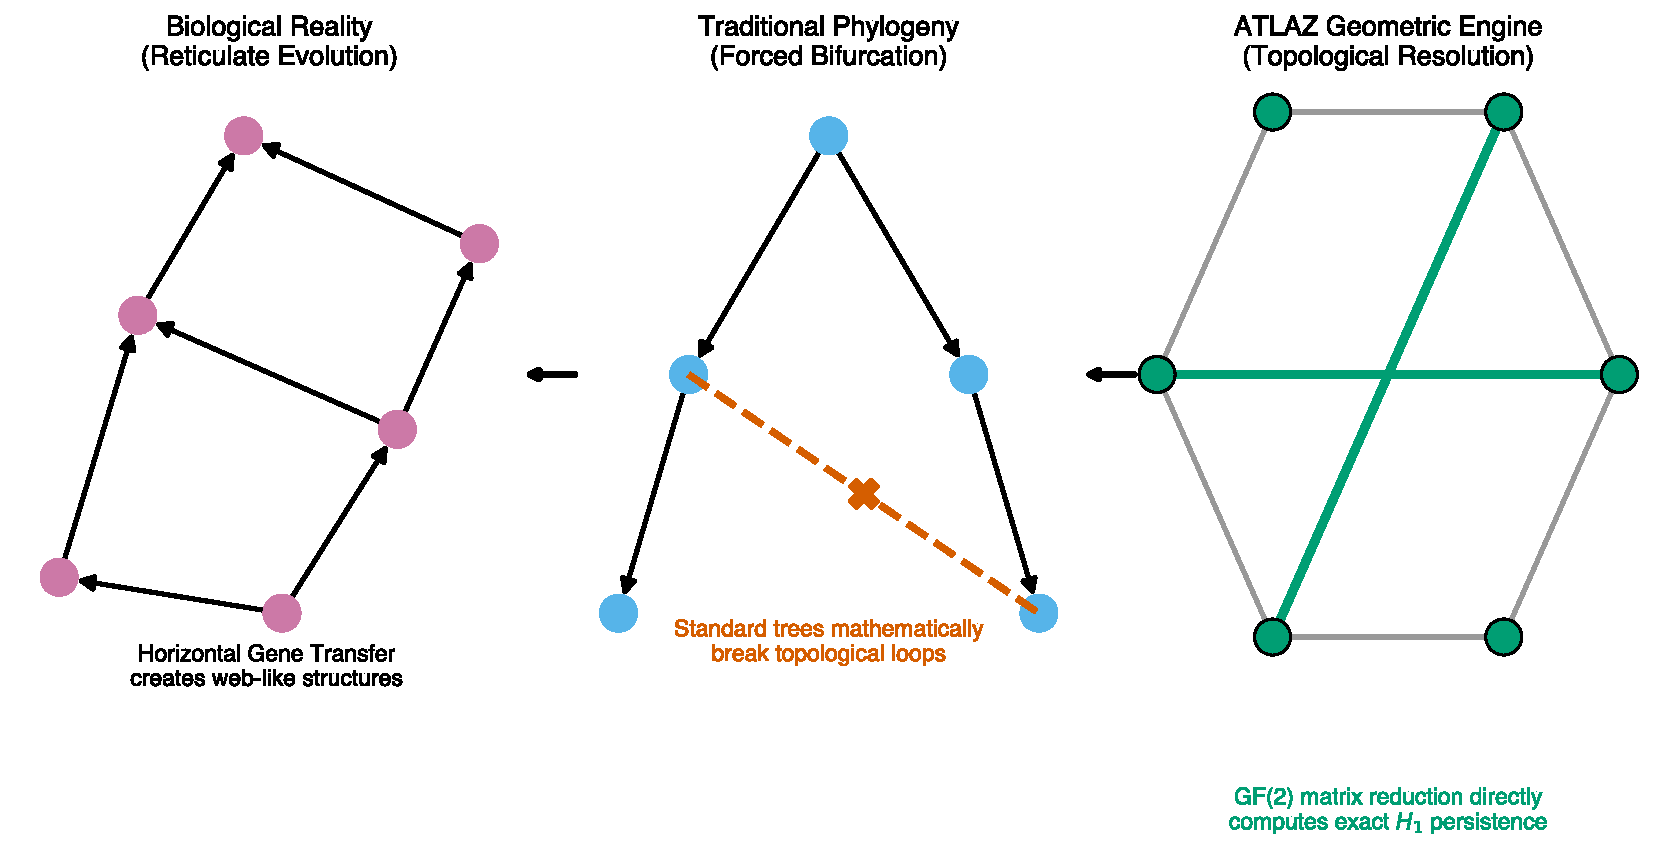
\includegraphics[width=\textwidth]{figures/graphical_abstract.pdf}
    \caption{\textbf{Graphical Abstract: Resolving the Bifurcation Constraint.} Traditional phylogenetic models (Panel A) force genomic lineages into strict bifurcating trees, leading to mathematical failures when presented with reticulate events like horizontal gene transfer or recombination. The ATLAZ geometric engine (Panel B) represents sequence space as a topological metric space, perfectly preserving $H_1$ homology loops and explicitly mapping evolutionary reticulation.}
    \label{fig:graphical_abstract}
\end{figure*}
